\section{Formal verification and validation}
\label{sec:formal_v_and_v}
Formal verification uses mathematical concepts to determine if a system satisfies requirements and operates as intended in all scenarios. Formal verification provides a high degree of assurance that the technology or system will function dependably in all circumstances, in contrast to routine testing, which examines particular scenarios. 

The proposed production system must undergo rigorous verification and validation  to guarantee its stability and reliability. With an emphasis on vital quality features like availability and integrity, this section describes the methodology for comparing the system's behavior to the main criteria.\cite{formalverification}

To evaluate our software system, we must test if the specified requirements are satisfied. The reason for conducting formal verification at this point of the project was to verify and mitigate potential errors made in the design level of the product line. This can save a lot of development time since errors identified earlier can be fixed much easier rather than identifying them in the later phases of the project.

UPPAAL is an effective tool for employing timed automata to describe, simulate, and validate the functioning of real-time systems. It is perfect for verifying systems where schedule and dependability is crucial since it enables users to examine system characteristics like fault tolerance and timing limitations. Using temporal logic specifications, we use UPPAAL to evaluate and validate the system model against these criteria, and ensure that the system fulfills properties such as liveness, safety and avoids deadlocks.\cite{Uppaal} An example of a timed automata can be seen in \ref{fig:TimedAutomata}


 %A. Verification Goals
%The following are the main objectives of the verification process:
%1. Ensure System Resilience: The system should be able cope with errors, including component fails, with little interruption, allowing it to continue operating.

%. Support Dynamic Scaling: Within the time frame and effort limits, the system should make it easier to integrate new AGC instances.

The three figures \ref{fig:Productline} represents the production line in UPPAAL. It's split into the user, who has two options of interaction with the system, namely starting production and requesting a database lookup, our HMI and a model of the AGC which subscribes the message bus. This model allows 
\begin{figure}[ht]
  \centering
  \begin{subfigure}[b]{0.4\linewidth}
    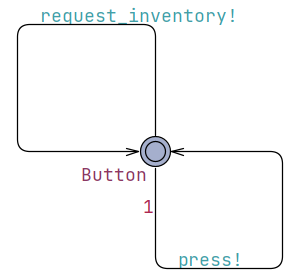
\includegraphics[width=\linewidth]{images/User.png}
     \caption{User}
  \end{subfigure}
  \begin{subfigure}[b]{0.5\linewidth}
    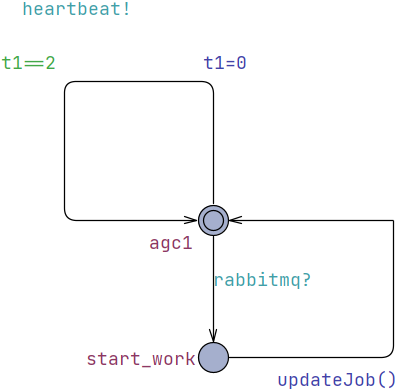
\includegraphics[width=\linewidth]{images/AGC.png}
    \caption{AGC}
  \end{subfigure}
  \begin{subfigure}[b]{0.7\linewidth}
    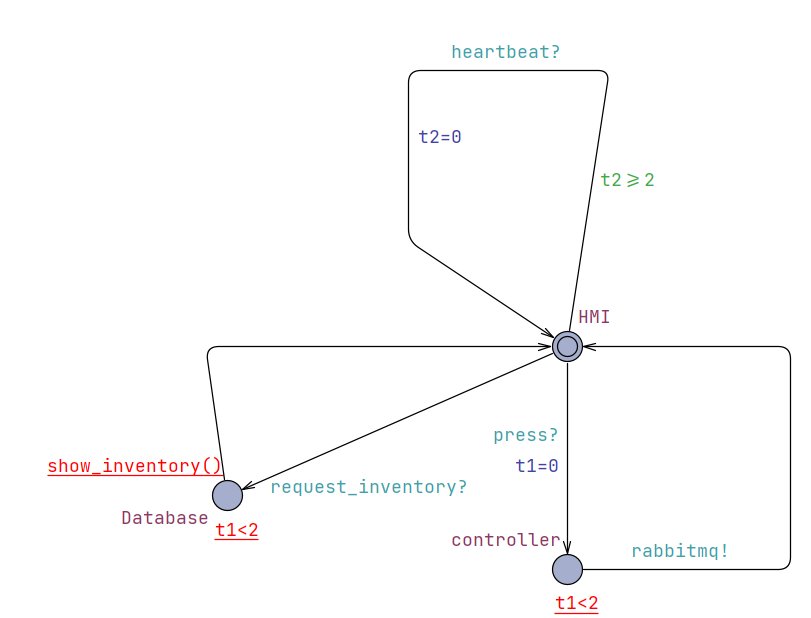
\includegraphics[width=\linewidth]{images/HMI.png}
    \caption{HMI}
  \end{subfigure}
  \caption{Formal verification model of production line}
  \label{fig:Productline}
\end{figure}




\ref{fig:Productline} is a specification of the vital parts of the product line system which can be formally verified. Most of the queries that are verified are directly corresponding to the requirements specified in \ref{tab:uppaal_queries} as seen by their id. The first query to be verified ensures that there are no deadlocks occurring in our behavioral model of the Product line. The second query from the Controller of the HMI to the AGC is a query that verifies the liveness of our system guaranteeing that, starting from the Controller state, the system will eventually reach AGC.start\_work which is the state in which the service subscribed to the message bus has received the signal to start production. This query corresponds to req\#5 from the previous section. The third query verifies that the AGC service, from receiving a message, will eventually reach back to the initial state agc1, meaning that the job has finished. The fourth query which checks for liveness between the AGC receiving the order, to finishing it, was not verifiable. The remaining queries ensure that all the states vital are reachable, and eventually return to the initial state where all actions start from. 


\begin{table}[ht]
\centering
\begin{tabular}{|p{4.5cm}|c|c|}
\hline
Query & Status & ReqId \\ \hline
A[] not deadlock & Verified & Req\#1 \\ \hline
$HMI.controller \rightarrow $AGC.start\_work & Verified &  Req\#5 \\ \hline
$A<> $AGC.start\_work and $jobsStart>=$1 imply AGC.agc1 & Verified & - \\ \hline
$AGC.start\_work \rightarrow $AGC.agc1   & Not Verified  & - \\ \hline
$E<> $HMI.Database  & Verified & Req\#4.1 \\ \hline
$HMI.controller \rightarrow $HMI.HMI & Verified  &Req\#6 \\ \hline
$HMI.Database \rightarrow $HMI.HMI & Verified & Req\#6.1 \\ \hline
\end{tabular}
\caption{UPPAAL queries}
\label{tab:uppaal_queries}
\end{table}
